
\section{Linearization procedure}

\red{
	O problema a ser resolvido � controlar um continuous-time switched affine system no formato:
	\begin{equation}
		\label{eq_continuous_time_dynamics}
		\dot{x}(t) = A_{\sigma(t)} x(t) + b_{\sigma(t)} 
	\end{equation}
	e o controle atua sobre o instante de atuacao do sinal de controle referencia, fazendo com que o sistema passe a ser n�o linear.
}

\begin{figure}[h]
	\centering
	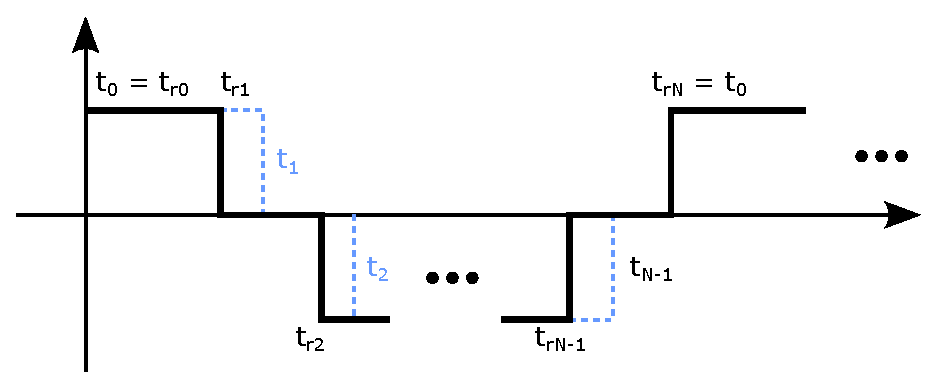
\includegraphics[]{Cap2/.fig/linearizacao_1.eps}
	\caption{Instantes de chaveamento}\label{cap2_linearizacao}
\end{figure}

% ========================= INSTANDE DE TEMPO 1 =========================
% =======================================================================

The solution fo the state equation \eqref{eq_continuous_time_dynamics} at time $t_N$, starting from the initial condition $x(t_0)$, is of the form

\begin{align}
	\label{eq_cap2_lin_x1}
	x(t_1)  &= e^{A_0(t_1-t_0)}x(t_0) + \intlinAA{0}{1}{}{} \\
	\label{eq_cap2_lin_xr1}
	x(t_{r_1}) &= e^{A_0(t_{r_1}-t_{r_0})}x(t_{r_0}) + \intlinA{0}{1}{r}{r}
\end{align}

subtracting \eqref{eq_cap2_lin_x1} and \eqref{eq_cap2_lin_xr1} we get

\begin{equation}
	\label{eq_cap2_lin_erro_x0x1}
	\begin{split}
		x(t_1) - x(t_{r_1}) = \overbrace{\green{e^{A_0(t_1-t_0)}x(t_0) - e^{A_0(t_{r_1}-t_{r_0})}x(t_{r_0})}}^{\green{\square}} \\
		+ \underbrace{\orange{\intlinAA{0}{1}{}{} - \intlinA{0}{1}{r}{r}}}_{\orange{\bigcirc}}
	\end{split}
\end{equation}

expanding $\green{\square}$

% 2.4
\begin{align}
  \green{\square} &= \green{e^{A_0(t_1-t_0)}x(t_0) - e^{A_0(t_{r_1}-t_{r_0})}x(t_{r_0})} \nonumber \\
				  &= \green{e^{A_0(t_{r_1} + \delta t_1 - t_0)}x(t_0) - e^{A_0(t_{r_1}-t_{r_0})}x(t_{r_0})} \nonumber \\
				  &= \blue{e^{A_0(t_{r_1} - t_0)}} \green{e^{\delta t_1} x(t_0)} \green{-} \blue{e^{A_0(t_{r_1}-t_{r_0})}}\green{x(t_{r_0})} \nonumber \\
				  &= \blue{F_{r_0}} \purple{e^{\delta t_1}} \green{x(t_0)} \green{-} \blue{F_{r_0}}\green{x(t_{r_0})} \nonumber \\
				  &= \green{F_{r_0}} \purple{(I + A_0 \delta t_1)} \green{x(t_0)} \green{-} \green{F_{r_0}}\green{x(t_{r_0})} \nonumber \\ 
				  \label{eq_cap2_lin_erro_x0x1_green}
				  &= \green{F_{r_0} [x(t_0) - x_r(t_0)] + F_{r_0} A_0 \delta t_1}
\end{align}

expanding $\orange{\bigcirc}$

% 2.5
\begin{align}
  \orange{\bigcirc} 	&= \orange{ \intlinAA{0}{1}{}{} - \intlinA{0}{1}{r}{r} } \nonumber \\ 
				   	&= \orange{ \intlinC{t_0}{t_{r_1}+\delta t_1}{0}{1} - \intlinA{0}{1}{}{r} } \nonumber \\
				   	&= \orange{ e^{A_0 \delta t_1} \bigg[ \blue{\intlinA{0}{1}{}{r}} + \purple{\intlinB{t_{r_1}}{t_{r_1} + \delta t_1}{0}{1}} \bigg] }
				   	   \orange{ -\blue{\intlinA{0}{1}{}{r}} } \nonumber \\
				   	&= \orange{ \pink{e^{A_0 \delta t_1}} [ \blue{G_{r_0}} + \purple{B_0 \delta t_1} ] - \blue{G_{r_0}} } \nonumber \\
				   	&= \orange{ \pink{(I + A_0 \delta t_1)}[ G_{r_0} + B_0 \delta t_1 ] - G_{r_0} } \nonumber \\
				   	&= \orange{ \cancel{G_{r_0}} + B_0 \delta t_1 + A_0 G_{r_0} \delta t_1 + \cancel{A_0 B_0 \delta t_1 \delta t_1} - \cancel{G_{r_0}} } \nonumber \\
					\label{eq_cap2_lin_erro_x0x1_orange}
				   	&= \orange{ A_0 G_{r_0} \delta t_1 + B_0 \delta t_1 }
\end{align}

and replacing \eqref{eq_cap2_lin_erro_x0x1_green} and \eqref{eq_cap2_lin_erro_x0x1_orange} into equation \eqref{eq_cap2_lin_erro_x0x1} we get to a equation that computes $x(t_1) - x_r(t_{r_1})$ from $x(t_0) - x_r(t_{r_0})$

\begin{equation}
	\label{eq_cap2_lin_erro_x0x1_resultado}
	x(t_1) - x_r(t_{r_1}) = F_{r_0} [ x(t_0) - x_r(t_0) ] + [ F_{r_0} A_0 x(t_0) + A_0 G_{r_0} + B_0 ] \delta t_1
\end{equation}
% ========================= INSTANDE DE TEMPO 2 =========================
% =======================================================================
Repeating the proceadure for $x(t_2)$ we have

\begin{align}
	\label{eq_cap2_lin_x2}
	x(t_2)  &= e^{A_1(t_2-t_1)}x(t_1) + \intlinAA{1}{2}{}{} \\
	\label{eq_cap2_lin_xr2}
	x(t_{r_2}) &= e^{A_1(t_{r_2}-t_{r_1})}x(t_{r_1}) + \intlinA{1}{2}{r}{r}
\end{align}

subtracting \ref{eq_cap2_lin_x2} and \ref{eq_cap2_lin_xr2} 

\begin{equation}
	\label{eq_cap2_lin_erro_x1x2}
	\begin{split}
		x(t_2) - x(t_{r_2}) = 
		\overbrace{\green{e^{A_1(t_2-t_1)}x(t_1) - e^{A_1(t_{r_2}-t_{r_1})}x(t_{r_1})}}^{\green{\square}} \\ 
		+ \underbrace{\orange{\intlinAA{1}{2}{}{} - \intlinA{1}{2}{r}{r}}}_{\orange{\bigcirc}}
	\end{split}
\end{equation}

expanding $\green{\square}$

% 2.10
\begin{align}
	\green{ \square } &=
	\green{
		e^{A_1(t_{r_2} + \delta t_2 - t_{r_1} - \delta t_1)} x(t_1)
		- e^{A_1(t_{r_2} - t_{r_1})} x_r(t_{r_1})
	} \nonumber \\
	&= \green{
		\blue{\Fri{1}{2}} \purple{e^{A_1(\delta t_2 - \delta t_1)}} x(t_1)
		- \blue{\Fri{1}{2}} x_r(t_{r_1})
	} \nonumber \\
	&= \green{
		\blue{F_{r_1}} \purple{[I + A_1(\delta t_2 - \delta t_1)]} x(t_1)
		- \blue{F_{r_1}} x_r(t_{r_1})
	} \nonumber \\
	\label{eq_cap2_lin_x2_green}
	&= \green{
		F_{r_1} [x(t_1) - x_r(t_{r_1})] + F_{r_1} A_1 x(t_1) \delta t_2
		- F_{r_1} A_1 x(t_1) \delta t_1
	}
\end{align}

expanding $\orange{\bigcirc}$

% 2.11
\begin{align}
	\orange{\bigcirc} 	&= \orange{\intlinAA{1}{2}{}{} - \intlinA{1}{2}{r}{r}} \nonumber \\
					   	&= \orange{ \intlinC{t_{r_1}+\delta t_1}{t_{r_2}+\delta t_2}{1}{2} - \intlinA{1}{2}{r}{r}} \nonumber \\
						\begin{split}
							&= \orange{ \purple{ e^{A_1 \delta t_2} }
								\bigg[
									\blue{\intlinA{1}{2}{r}{r}} - \intlinB{t_{r_1}}{t_{r_1} + \delta t_1}{1}{2} + \intlinB{t_{r_2}}{t_{r_2} + \delta t_2}{1}{2} \bigg] } \\
							& \qquad \orange{ - \blue{\intlinA{1}{2}{r}{r}} }
						\end{split} \nonumber \\
						&= \orange{ \purple{(I + A_1 \delta t_2)}
							\bigg[
								\blue{G_{r_1}} - \pink{\intlinB{t_{r_1}}{t_{r_1} + \delta t_1}{1}{2}} + \brown{\intlinB{t_{r_2}}{t_{r_2} + \delta t_2}{1}{2}}
							\bigg] - \blue{G_{r_1}}
						} \nonumber \\
						&= \orange{ (I + A_1 \delta t_2)
							\bigg[
								G_{r_1} - \pink{e^{A_1(t_{r_2} - t_{r_1})} B_1 \delta t_1} + \brown{B_1 \delta t_2}
							\bigg] - G_{r_1}
						} \nonumber \\
						&= \orange{ (I + A_1 \delta t_2)
							\bigg[
								G_{r_1} - \pink{F_{r_1} B_1 \delta t_1} + B_1 \delta t_2
							\bigg] - G_{r_1}
						} \nonumber \\
						&= \orange{ \cancel{G_{r_1}} - F_{r_1} B_1 \delta t_1 + B_1 \delta t_2 + A_1 G_{r_1} \delta t_2 - \cancel{G_{r_1}} } \nonumber \\
						\label{eq_cap2_lin_x2_orange}
						&= \orange{ A_1 G_{r_1} \delta t_2 + B_1 \delta t_2 - F_{r_1} B_1 \delta t_1 }
\end{align}

replacing (\ref{eq_cap2_lin_x2_green}) and (\ref{eq_cap2_lin_x2_orange}) into equation (\ref{eq_cap2_lin_erro_x1x2})
\begin{equation}
	\label{eq_xt2_xt1_0}
	\begin{split}
		x(t_2) - x_r(t_{r_2}) =  & F_{r_1} [\green{x(t_1) - x_{r_1}(t_{r_1})}] \\
							     & \quad - F_{r_1} [A_1 \blue{x(t_1)} + B_1] \delta t_1 \\
							     & \quad + [ F_{r_1} A_1 \underbrace{\blue{x(t_1)}}_{\blue{\triangle}} + A_1 G_{r_1} + B_1] \delta t_2
	\end{split} 
\end{equation}

expanding $\blue{\triangle}$ from \ref{eq_cap2_lin_erro_x0x1_resultado}

\begin{equation}
	\blue{\triangle} = x(t_1) = x_r(t_{r_1}) + F_{r_0} [ x(t_0) - x_r(t_0) ] + [ F_{r_0} A_0 x(t_0) + A_0 G_{r_0} + B_0 ] \delta t_1 
	\nonumber
\end{equation}

note that when $\blue{\triangle}$ is replaced in eq. \ref{eq_xt2_xt1_0} it will produce a product with $\delta t_1$ and $\delta t_2$ like
\begin{equation}
	x(t_1)\delta t_1 = x_r(t_{r_1})\delta t_1 + F_{r_0} \red{\overbrace{ [ x(t_0) - x_r(t_0) ]\delta t_1 }^{\square}} + [ F_{r_0} A_0 x(t_0) + A_0 G_{r_0} + B_0 ] \purple{\overbrace{\delta t_1\delta t_1}^{\bigcirc}} 
	\nonumber
\end{equation}

both $\red{\square}$ and $\purple{\bigcirc}$ are products of diferences that produces a smaller number and they will computed as $\approx 0$

\begin{equation}
	\label{eq_xt1_deltat1_aprox}
	x(t_1)\delta t_1 \approx x_r(t_{r_1})\delta t_1 
\end{equation}

replacing equation \ref{eq_cap2_lin_erro_x0x1_resultado} and \ref{eq_xt1_deltat1_aprox} in \ref{eq_xt2_xt1_0}
\begin{equation}
	\begin{split}
		x(t_2) - x_r(t_{r_2}) =  & F_{r_1} \{\green{
										F_{r_0} [x(t_0) - x_r(t_0) + [F_{r_0} A_0 x(t_0) + A_0 G_{r_0} + B_0] \delta t_1]
								 }\} \\
							     & \quad - F_{r_1} [A_1 \blue{x_r(t_1)} + B_1] \delta t_1 \\
							     & \quad + [ F_{r_1} A_1 \blue{x_r(t_1)} + A_1 G_{r_1} + B_1] \delta t_2
	\end{split}
	\nonumber
\end{equation}
\begin{equation}
	\begin{split}
		x(t_2) - x_r(t_{r_2}) =  & F_{r_1} F_{r_0} [x(t_0) - x_r(t_0)] \\
							     & \quad + F_{r_1} [F_{r_0} A_0 x(t_0) + A_0 G_{r_0} - A_1 x_r(t_{r_1}) + B_0 - B_1] \delta t_1 \\
							     & \quad + [F_{r_1} A_1 x_r(t_{r_1}) + A_1 G_{r_1} + B_1] \delta t_2
	\end{split}
\end{equation}
\input{Cap3/cap3_lin_instante3}
% ========================= INSTANDE DE TEMPO i =========================
% =======================================================================

Continuing on expanding the propagation of the system further more we can deduce the equation for $x(t_i)$ as
% 2.21
\begin{align}
	\begin{split}
		x(t_i) - x_r(t_{r_i}) =  & F_{r_{i-1}}F_{r_{i-2}} \ldots F_{r_0} [x(t_0) - x_r(t_0)] \\
								 & + F_{r_{i-1}}F_{r_{i-2}} \ldots F_{r_1} [F_{r_0} A_0 x(t_0) + A_0 G_{r_0} - A_1 x_r(t_{r_1}) + B_0 - B_1] \delta t_1 \\
								 & + F_{r_{i-1}}F_{r_{i-2}} \ldots F_{r_2} [F_{r_1} A_1 x(t_1) + A_1 G_{r_1} - A_2 x_r(t_{r_2}) + B_1 - B_2] \delta t_2 \\
								 & \qquad \vdots \\
								 & + F_{r_{i-1}}[F_{r_{i-2}} A_{i-2} x_r(t_{i-2}) + A_{i-2} G_{r_{i-2}} - A_{i-1} x_r(t_{r_{i-1}}) + B_{i-2} - B_{i-1} ] \delta t_{i-1} \\
							     & + [F_{r_{i-1}} A_{i-1} x_r(t_{i-1}) + A_{i-1} G_{r_{i-1}} + B_{i-1}] \delta t_i
	\end{split}
\end{align}

% ========================= INSTANDE DE TEMPO N =========================
% =======================================================================

and then, for $x(t_N)$ we have 

% 2.22
\begin{align}
	\label{eq_xN_propagation}
		x(t_N) - x_r(t_{r_N}) =  & F_{r_{N-1}}F_{r_{N-2}} \ldots F_{r_0} [x(t_0) - x_r(t_0)] \nonumber \\
								 & + F_{r_{N-1}}F_{r_{N-2}} \ldots F_{r_1} [\overbrace{\green{F_{r_0} A_0 x(t_0) + A_0 G_{r_0} - A_1 x_r(t_{r_1}) + B_0 - B_1}}^{\green{\square}}] \delta t_1 \nonumber \\
								 & + F_{r_{N-1}}F_{r_{N-2}} \ldots F_{r_2} [\green{F_{r_1} A_1 x(t_1) + A_1 G_{r_1} - A_2 x_r(t_{r_2}) + B_1 - B_2}] \delta t_2 \nonumber \\
								 & \qquad \vdots \nonumber \\
								 \begin{split}
									& + F_{r_{N-1}}[\green{F_{r_{N-2}} A_{N-2} x_r(t_{N-2}) + A_{N-2} G_{r_{N-2}} - A_{N-1} x_r(t_{r_{N-1}})} \\ 
									& \qquad \qquad \qquad \green{+ B_{N-2} - B_{N-1}} ] \delta t_{N-1}
								 \end{split} \nonumber \\
							     & + [\underbrace{\orange{F_{r_{N-1}} A_{N-1} x_r(t_{N-1}) + A_{N-1} G_{r_{N-1}} + B_{N-1}}}_{\orange{\bigcirc}}] \delta t_N
\end{align}

% 2.23
\begin{align}
	\label{eq_square_xN}
	\green{\square} &= \green{F_{r_0} A_0 x(t_0) + A_0 G_{r_0} - A_1 x_r(t_{r_1}) + B_0 - B_1} \nonumber \\
					&= \green{A_0 \purple{F_{r_0} x(t_0)} + A_0 G_{r_0} - A_1 x_r(t_{r_1}) + B_0 - B_1} \nonumber \\
					&= \green{A_0 \purple{[x_r(t_{r_1}) - G_{r_0}]} + A_0 G_{r_0} - A_1 x_r(t_{r_1}) + B_0 - B_1} \nonumber \\
					&= \green{A_0 x_r(t_{r_1}) - \cancel{A_0 G_{r_0}} + \cancel{A_0 G_{r_0}} - A_1 x_r(t_{r_1}) + B_0 - B_1} \nonumber \\
					&= \green{(A_0 - A_1) x_r(t_{r_1}) + B_0 - B_1}
\end{align}

% 2.24
\begin{align}
	\label{eq_circle_xN}
	\orange{\bigcirc} &= \orange{F_{r_{N-1}} A_{N-1} x_r(t_{N-1}) + A_{N-1} G_{r_{N-1}} + B_{N-1}} \nonumber \\
					 &= \orange{A_{N-1} \purple{F_{r_{N-1}} x_r(t_{N-1})} + A_{N-1} G_{r_{N-1}} + B_{N-1}} \nonumber \\
					 &= \orange{A_{N-1} \purple{[x_r(t_{r_N}) - G_{r_{N-1}}]} + A_{N-1} G_{r_{N-1}} + B_{N-1}} \nonumber \\
					 &= \orange{A_{N-1} x_r(t_{r_N}) - \cancel{A_{N-1} G_{r_{N-1}}} + \cancel{A_{N-1} G_{r_{N-1}}} + B_{N-1}} \nonumber \\
					 &= \orange{A_{N-1} x_r(t_{r_N}) + B_{N-1}}
\end{align}

replacing \ref{eq_square_xN} and \ref{eq_circle_xN} in \ref{eq_xN_propagation}

\begin{align}
	\begin{split}
		x(t_N) - x_r(t_{r_N}) =  & \quad F_{r_{N-1}}F_{r_{N-2}} \ldots F_{r_0} [x(t_0) - x_r(t_0)] \\
								 & + F_{r_{N-1}}F_{r_{N-2}} \ldots F_{r_1} [\green{(A_0 - A_1) x_r(t_{r_1}) + B_0 - B_1}] \delta t_1 \\
								 & + F_{r_{N-1}}F_{r_{N-2}} \ldots F_{r_2} [\green{(A_1 - A_2) x_r(t_{r_2}) + B_1 - B_2}] \delta t_2 \\
								 & \qquad \vdots \\
								 & + F_{r_{N-1}}[\green{(A_{N-2} - A_{N-1}) x_r(t_{r_{N-1}}) + B_{N-2} - B_{N-1}}] \delta t_{N-1} \\
							     & + [\orange{A_{N-1} x_r(t_{r_N}) + B_{N-1}}] \delta t_N
	\end{split}
\end{align}

\begin{align}
	e(t) &= x(t) - x_r(t_r) \\ \nonumber \\
	\Phi &= F_{r_{N-1}} F_{r_{N-2}} \ldots F_{r_0} \\ \nonumber \\
	\begin{split}
		\Gamma &= \Big[ F_{r_{N-1}}F_{r_{N-2}} \ldots F_{r_1} [(A_0 - A_1) x_r(t_{r_1}) + B_0 - B_1], \\
		& \qquad F_{r_{N-1}}F_{r_{N-2}} \ldots F_{r_2} [(A_1 - A_2) x_r(t_{r_2}) + B_1 - B_2], \\
		& \qquad \qquad \vdots \\
		& \qquad F_{r_{N-1}}[(A_{N-2} - A_{N-1}) x_r(t_{r_{N-1}}) + B_{N-2} - B_{N-1}]\Big]
	\end{split} \\ \nonumber \\
	\delta t &= [\delta t_1, \delta t_2, \ldots, \delta t_N]^T \\ \nonumber \\
	e(t_N) &= \Phi e(t_0) + \Gamma \delta t
\end{align}

where $x_r$ is calculated as
\begin{align}
	x_r(t_{r_1}) &= F_0 x_r(t_{r_0}) + G_0 \\
    x_r(t_{r_2}) &= F_1 x_r(t_{r_1}) + G_1 \\
    &\vdots \nonumber \\
    x_r(t_{r_N}) &= F_{N-1} x_r(t_{r_{N-1}}) + G_{N-1}
\end{align}

and $F_i$ and $G_i$ are calculated as

\begin{equation}
	[F_i, G_i] = c2dm(Ai, Bi, [], [], dti, `zoh`)
\end{equation}